\newpage
\section{}

\subsection{a}

lrs = [0.001, 0.01, 0.03, 0.04, 0.05]
momentums = [0.5, 0.7, 0.9]
Ms = [128, 256, 512, 1024, 2048]
momentum =[20, 60, 100]

I used the combination of random and grid search, I first hand searched
few number and found out the higher momentum and learning rate around 
0.03 with momentum over 60 has the best validation accuracy. After I have a sense of 
how accuracy is affected, then I grid searched the hyperparameters and found
below are the three best models performance.

\begin{figure}[!ht]
    \centering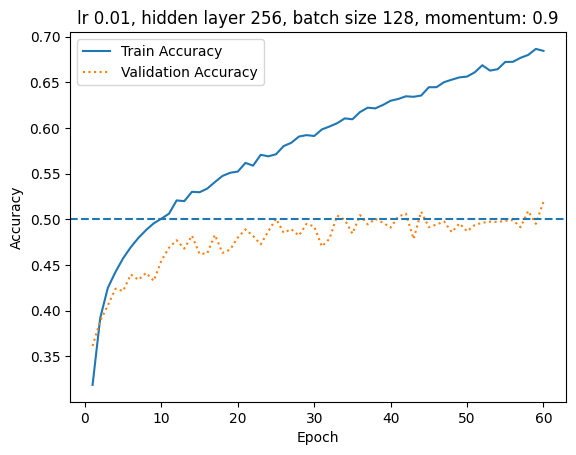
\includegraphics[width=1\linewidth]{A5-0.png}
    \caption{accuracy: 0.512}
\end{figure}


\begin{figure}[!ht]
    \centering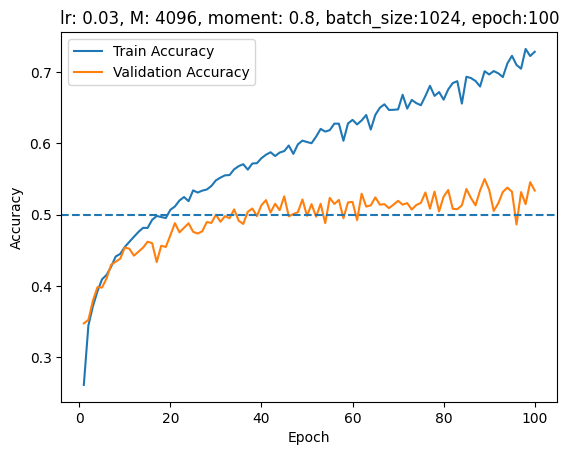
\includegraphics[width=1\linewidth]{A5-1.png}
    \caption{accuracy: 0.532}
\end{figure}


\begin{figure}[!t]
    \centering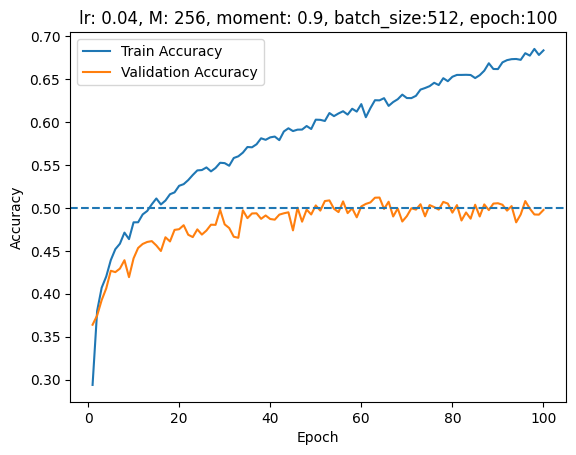
\includegraphics[width=1\linewidth]{A5-2.png}
    \caption{accuracy: 0.503}
\end{figure}




\clearpage

\subsection{b}
searched over parameters
lrs = [0.001, 0.01]
momentums = [0.5, 0.7, 0.9]
Ms = [64, 128, 256]
ks = [3, 5, 7]
Ns = [2, 4, 7]

I used grid search, I used for loop to find the combinatorial of all
posible hyperparameter pair and searched the best performing model.

\begin{figure}[!ht]
    \centering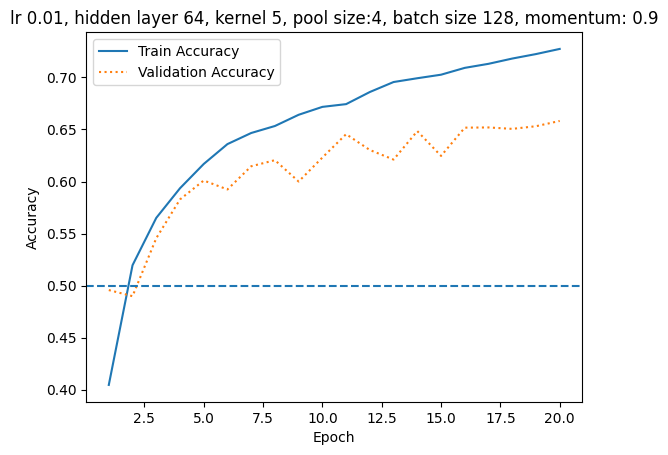
\includegraphics[width=1\linewidth]{A5b-0.png}
    \caption{accuracy: 0.634}
\end{figure}

\begin{figure}[!ht]
    \centering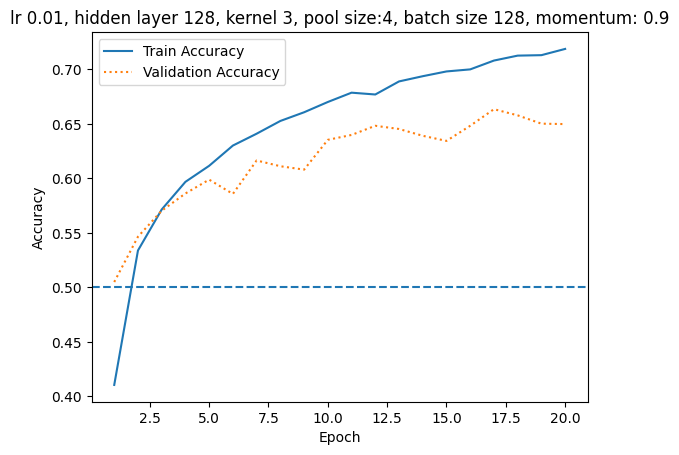
\includegraphics[width=1\linewidth]{A5b-1.png}
    \caption{accuracy: 0.63}
\end{figure}
\begin{figure}[!t]
    \centering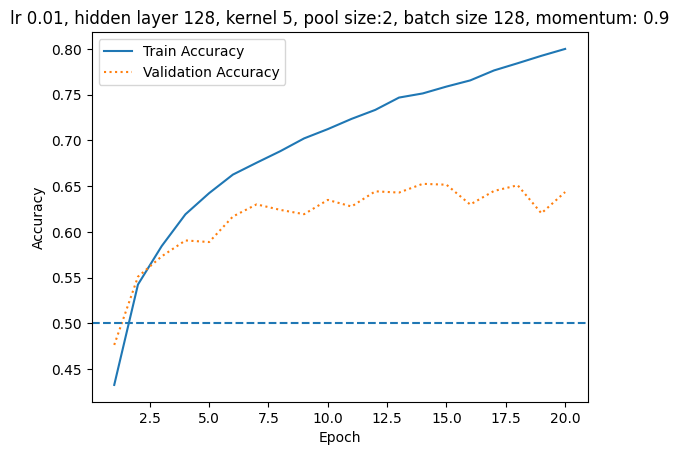
\includegraphics[width=1\linewidth]{A5b-2.png}
    \caption{accuracy: 0.623}
\end{figure}

\newpage
\inputminted{python3}{../hw4-A/image_classification.py}